% !TEX root = ../agglo_clust_review.tex



% \begin{figure*}[htp]
% \captionsetup{font=small}
% \hspace*{\fill}
% \begin{minipage}[t]{0.38\textwidth}
% \centering
% \vspace{0pt}
%         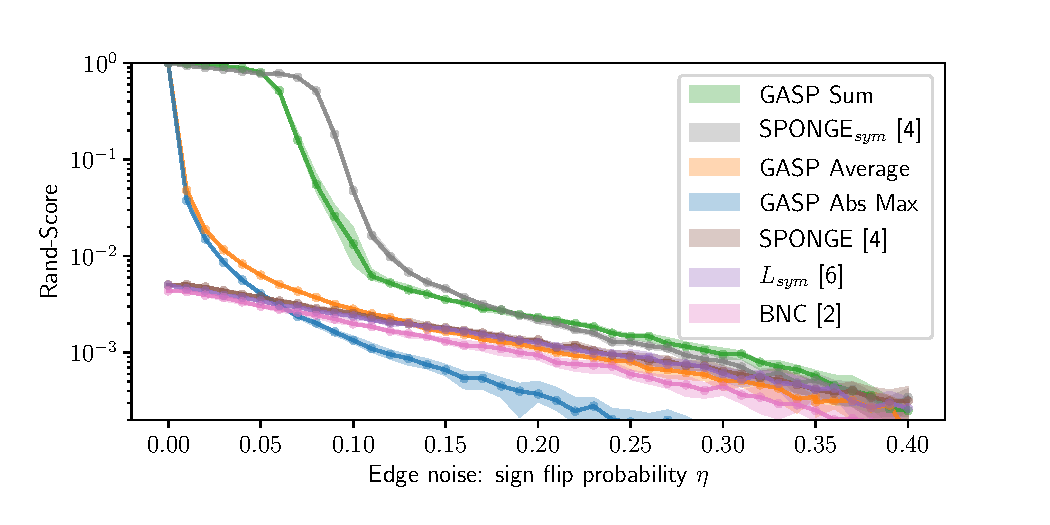
\includegraphics[width=\textwidth,trim=0.25in 0.25in 0.68in 0.36in,clip]{./figs/SSBM_experiments.pdf}
%         \captionof{figure}{Experiments on SSBM synthetic graphs}
%     \label{fig:SSBM_experiments}
% \end{minipage}\hfill
% \begin{minipage}[t]{0.25\textwidth}
% \centering
% \vspace{0pt}
%     \scriptsize
% \begin{tabular}{l|c}
%            Method & Rand-Score \\ \midrule
%            \textbf{GASP Average} & \textbf{0.8966} \\
% GASP Sum & 0.8965 \\
% GASP Abs Max & 0.8932 \\
% SPONGE$_{sym}$ \cite{Cucuringu2019SPONGEAG} & 0.5839\\
% $L_{sym}$ \cite{kunegis2010spectral} & 0.1931 \\
% SPONGE \cite{Cucuringu2019SPONGEAG} & 0.0789 \\
% BNC \cite{chiang2012scalable} & 0.0074 \\
%         \end{tabular}
%     \captionof{table}{Experiments on a tiny crop of the CREMI dataset, training sample B.}
%     \label{tab:cremi_experiments}
% \end{minipage}
% \end{figure*}

\begin{figure}[t]
\centering
\begin{minipage}[t]{\textwidth}
\vspace{0pt}
\centering
% \footnotesize
\begin{tabular}[t]{L{29em} M{7em}}
           Method & Rand-Score \\ \midrule
           \textbf{GASP Average} & \textbf{0.8966} \\
GASP Sum & 0.8965 \\
GASP Abs Max & 0.8932 \\
SPONGE$_{sym}$ \cite{Cucuringu2019SPONGEAG} & 0.5839\\
$L_{sym}$ \cite{kunegis2010spectral} & 0.1931 \\
SPONGE \cite{Cucuringu2019SPONGEAG} & 0.0789 \\
BNC \cite{chiang2012scalable} & 0.0074 \\
        \end{tabular}
    \captionof{table}{\algname{} compared to spectral clustering methods on a small crop of the CREMI dataset (sample B).}
    \label{tab:cremi_spectral_experiments}
\end{minipage}\\\vspace{2em}
\begin{minipage}[t]{\textwidth}
\vspace{0pt}
\centering
        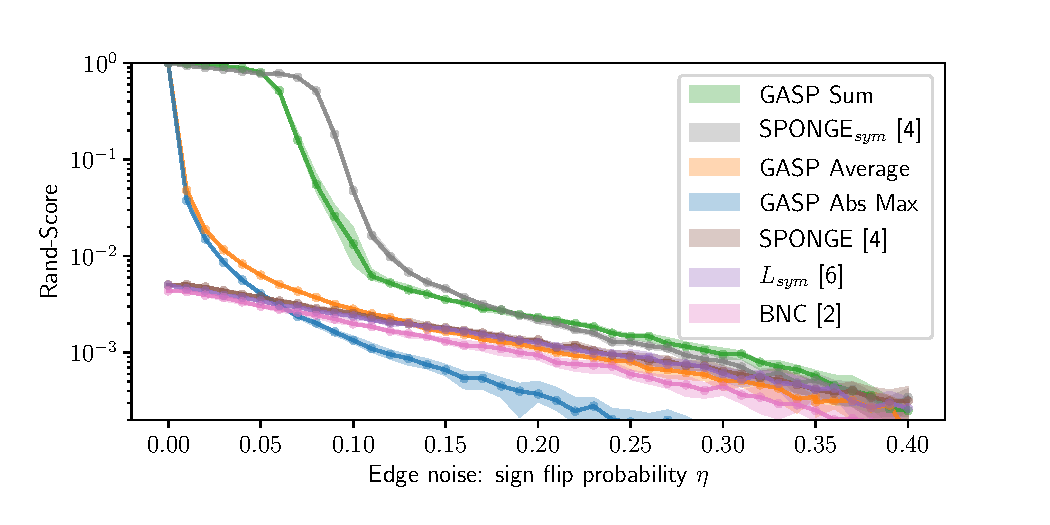
\includegraphics[width=0.8\textwidth,trim=0.25in 0.25in 0.68in 0.36in,clip]{./figs/SSBM_experiments.pdf} % 0.45
        \caption{\algname{} performances compared to spectral methods on synthetic graphs. The spectral methods were given the true number of clusters as input, in contrast to \algname{}.}
    \label{fig:SSBM_spectral_experiments}
\end{minipage}
\end{figure}


\section{Comparison with spectral clustering} \label{sec:spectral_clust}
In this section we compare \algname{} to spectral clustering (SC) methods for signed graphs both on synthetic graphs and real ones from neuron segmentation. These methods require the user to specify the number of clusters in advance, in contrast to our proposed agglomeration method that determines the cluster number based on the signed weights of the graph. In the following comparison, we make these baselines as strong as possible by specifying the true number of clusters for the spectral methods.

\textbf{Synthetic graphs} -- First, we compare the clustering performance on synthetic graphs generated by a signed stochastic block model (SSBM), where SC performs well. In particular, we used an Erd\H os-R\'enyi random graph model $\mathcal{G}(N,p)$ with $N=10^5$ vertices and edge probability $p=0.1$. Following the approach in \cite{Cucuringu2019SPONGEAG}, we partitioned the graph into $k=100$ equally-sized clusters, such that edges connecting vertices belonging to the same cluster (different clusters, respectively) had Gaussian distributed edge weights centered at $\mu=1$ ($\mu=-1$, respectively) and with standard deviation $0.1$. To model noise, we flipped the sign of each edge independently with probability $\eta \in [0, 0.4]$. Median scores, 25th and 75th percentiles over 30 repetitions are shown in Fig.~\ref{fig:SSBM_spectral_experiments}: GASP achieved scores comparable to SPONGE$_{sym}$ \cite{Cucuringu2019SPONGEAG}, a recently proposed SC method. The specific design choice of a \emph{sign flipping} noise used in the SSBM experiments turned out to favor GASP with \emph{Sum} linkage that, according to the experiments presented in Sec.~\ref{sec:results}, is the one with the lowest tendency to over-cluster and grows one cluster at the time.

\textbf{Neuron segmentation} -- We extended the comparison with spectral methods to the task of neuron segmentation. Since SC cannot scale to the full CREMI dataset, we evaluated \algname{} and SC on a smaller $10\times100\times100$ voxels volume resulting in a graph with $10^5$ nodes and~$\sim10^6$ edges. Scores are summarized in Table \ref{tab:cremi_spectral_experiments}.
%suggested by the reviewer that performed best in the recent comparison \cite{Cucuringu2019SPONGEAG}: one based on the Balanced Normalized Cut (BNC) \cite{chiang2012scalable}; another on the symmetrically normalized Signed Laplacian ($L_{sym}$) \cite{kunegis2010spectral}; SPONGE and SPONGE$_{sym}$ algorithms were recently proposed in \cite{Cucuringu2019SPONGEAG}.
Despite the fact that the true number of ground truth clusters was given as an input to the SC methods, GASP significantly outperformed them on neuro-data. SC methods seem to have more difficulties when the graph is sparse. Moreover, they did not handle well pixels on the boundaries between segments and tended to cluster them together. Increasing $k$ did not improve their scores either.



